% Created by tikzDevice version 0.6.2-92-0ad2792 on 2013-02-07 02:00:58
% !TEX encoding = UTF-8 Unicode
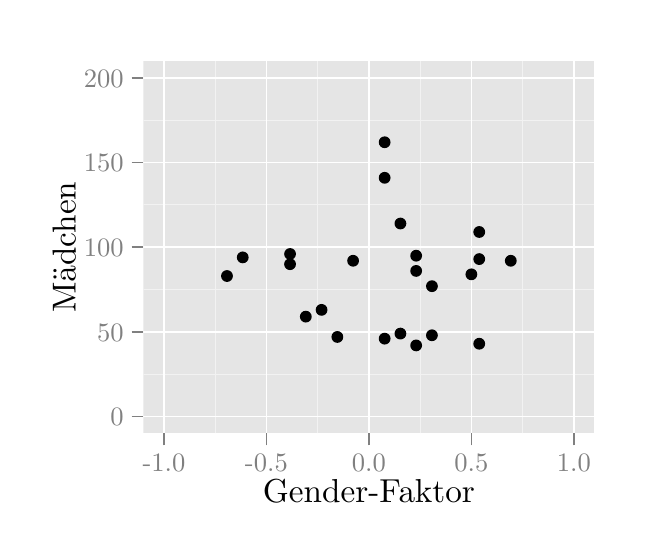
\begin{tikzpicture}[x=1pt,y=1pt]
\definecolor[named]{fillColor}{rgb}{1.00,1.00,1.00}
\path[use as bounding box,fill=fillColor,fill opacity=0.00] (0,0) rectangle (216.81,180.67);
\begin{scope}
\path[clip] (  0.00,  0.00) rectangle (216.81,180.67);
\definecolor[named]{drawColor}{rgb}{1.00,1.00,1.00}
\definecolor[named]{fillColor}{rgb}{1.00,1.00,1.00}

\path[draw=drawColor,line width= 0.6pt,line join=round,line cap=round,fill=fillColor] (  0.00,  0.00) rectangle (216.81,180.68);
\end{scope}
\begin{scope}
\path[clip] ( 41.82, 34.03) rectangle (204.77,168.63);
\definecolor[named]{fillColor}{rgb}{0.90,0.90,0.90}

\path[fill=fillColor] ( 41.82, 34.03) rectangle (204.77,168.63);
\definecolor[named]{drawColor}{rgb}{0.95,0.95,0.95}

\path[draw=drawColor,line width= 0.3pt,line join=round] ( 41.82, 55.45) --
	(204.77, 55.45);

\path[draw=drawColor,line width= 0.3pt,line join=round] ( 41.82, 86.04) --
	(204.77, 86.04);

\path[draw=drawColor,line width= 0.3pt,line join=round] ( 41.82,116.63) --
	(204.77,116.63);

\path[draw=drawColor,line width= 0.3pt,line join=round] ( 41.82,147.22) --
	(204.77,147.22);

\path[draw=drawColor,line width= 0.3pt,line join=round] ( 67.74, 34.03) --
	( 67.74,168.63);

\path[draw=drawColor,line width= 0.3pt,line join=round] (104.78, 34.03) --
	(104.78,168.63);

\path[draw=drawColor,line width= 0.3pt,line join=round] (141.81, 34.03) --
	(141.81,168.63);

\path[draw=drawColor,line width= 0.3pt,line join=round] (178.84, 34.03) --
	(178.84,168.63);
\definecolor[named]{drawColor}{rgb}{1.00,1.00,1.00}

\path[draw=drawColor,line width= 0.6pt,line join=round] ( 41.82, 40.15) --
	(204.77, 40.15);

\path[draw=drawColor,line width= 0.6pt,line join=round] ( 41.82, 70.74) --
	(204.77, 70.74);

\path[draw=drawColor,line width= 0.6pt,line join=round] ( 41.82,101.33) --
	(204.77,101.33);

\path[draw=drawColor,line width= 0.6pt,line join=round] ( 41.82,131.92) --
	(204.77,131.92);

\path[draw=drawColor,line width= 0.6pt,line join=round] ( 41.82,162.51) --
	(204.77,162.51);

\path[draw=drawColor,line width= 0.6pt,line join=round] ( 49.23, 34.03) --
	( 49.23,168.63);

\path[draw=drawColor,line width= 0.6pt,line join=round] ( 86.26, 34.03) --
	( 86.26,168.63);

\path[draw=drawColor,line width= 0.6pt,line join=round] (123.29, 34.03) --
	(123.29,168.63);

\path[draw=drawColor,line width= 0.6pt,line join=round] (160.33, 34.03) --
	(160.33,168.63);

\path[draw=drawColor,line width= 0.6pt,line join=round] (197.36, 34.03) --
	(197.36,168.63);
\definecolor[named]{fillColor}{rgb}{0.00,0.00,0.00}

\path[fill=fillColor] (111.90, 68.91) circle (  2.13);

\path[fill=fillColor] (117.59, 96.44) circle (  2.13);

\path[fill=fillColor] (128.99, 68.30) circle (  2.13);

\path[fill=fillColor] (128.99,139.26) circle (  2.13);

\path[fill=fillColor] (140.38, 65.85) circle (  2.13);

\path[fill=fillColor] (163.17,106.84) circle (  2.13);

\path[fill=fillColor] ( 77.71, 97.66) circle (  2.13);

\path[fill=fillColor] ( 94.81, 98.89) circle (  2.13);

\path[fill=fillColor] ( 94.81, 95.21) circle (  2.13);

\path[fill=fillColor] (174.57, 96.44) circle (  2.13);

\path[fill=fillColor] ( 72.02, 90.93) circle (  2.13);

\path[fill=fillColor] (100.50, 76.25) circle (  2.13);

\path[fill=fillColor] (106.20, 78.70) circle (  2.13);

\path[fill=fillColor] (128.99,126.42) circle (  2.13);

\path[fill=fillColor] (134.69,109.90) circle (  2.13);

\path[fill=fillColor] (134.69, 70.13) circle (  2.13);

\path[fill=fillColor] (163.17, 66.46) circle (  2.13);

\path[fill=fillColor] (146.08, 69.52) circle (  2.13);

\path[fill=fillColor] (140.38, 98.27) circle (  2.13);

\path[fill=fillColor] (140.38, 92.77) circle (  2.13);

\path[fill=fillColor] (146.08, 87.26) circle (  2.13);

\path[fill=fillColor] (160.33, 91.54) circle (  2.13);

\path[fill=fillColor] (163.17, 97.05) circle (  2.13);
\end{scope}
\begin{scope}
\path[clip] (  0.00,  0.00) rectangle (216.81,180.67);
\definecolor[named]{drawColor}{rgb}{0.50,0.50,0.50}

\node[text=drawColor,anchor=base east,inner sep=0pt, outer sep=0pt, scale=  0.96] at ( 34.71, 36.85) {0};

\node[text=drawColor,anchor=base east,inner sep=0pt, outer sep=0pt, scale=  0.96] at ( 34.71, 67.44) {50};

\node[text=drawColor,anchor=base east,inner sep=0pt, outer sep=0pt, scale=  0.96] at ( 34.71, 98.03) {100};

\node[text=drawColor,anchor=base east,inner sep=0pt, outer sep=0pt, scale=  0.96] at ( 34.71,128.62) {150};

\node[text=drawColor,anchor=base east,inner sep=0pt, outer sep=0pt, scale=  0.96] at ( 34.71,159.21) {200};
\end{scope}
\begin{scope}
\path[clip] (  0.00,  0.00) rectangle (216.81,180.67);
\definecolor[named]{drawColor}{rgb}{0.50,0.50,0.50}

\path[draw=drawColor,line width= 0.6pt,line join=round] ( 37.55, 40.15) --
	( 41.82, 40.15);

\path[draw=drawColor,line width= 0.6pt,line join=round] ( 37.55, 70.74) --
	( 41.82, 70.74);

\path[draw=drawColor,line width= 0.6pt,line join=round] ( 37.55,101.33) --
	( 41.82,101.33);

\path[draw=drawColor,line width= 0.6pt,line join=round] ( 37.55,131.92) --
	( 41.82,131.92);

\path[draw=drawColor,line width= 0.6pt,line join=round] ( 37.55,162.51) --
	( 41.82,162.51);
\end{scope}
\begin{scope}
\path[clip] (  0.00,  0.00) rectangle (216.81,180.67);
\definecolor[named]{drawColor}{rgb}{0.50,0.50,0.50}

\path[draw=drawColor,line width= 0.6pt,line join=round] ( 49.23, 29.77) --
	( 49.23, 34.03);

\path[draw=drawColor,line width= 0.6pt,line join=round] ( 86.26, 29.77) --
	( 86.26, 34.03);

\path[draw=drawColor,line width= 0.6pt,line join=round] (123.29, 29.77) --
	(123.29, 34.03);

\path[draw=drawColor,line width= 0.6pt,line join=round] (160.33, 29.77) --
	(160.33, 34.03);

\path[draw=drawColor,line width= 0.6pt,line join=round] (197.36, 29.77) --
	(197.36, 34.03);
\end{scope}
\begin{scope}
\path[clip] (  0.00,  0.00) rectangle (216.81,180.67);
\definecolor[named]{drawColor}{rgb}{0.50,0.50,0.50}

\node[text=drawColor,anchor=base,inner sep=0pt, outer sep=0pt, scale=  0.96] at ( 49.23, 20.31) {-1.0};

\node[text=drawColor,anchor=base,inner sep=0pt, outer sep=0pt, scale=  0.96] at ( 86.26, 20.31) {-0.5};

\node[text=drawColor,anchor=base,inner sep=0pt, outer sep=0pt, scale=  0.96] at (123.29, 20.31) {0.0};

\node[text=drawColor,anchor=base,inner sep=0pt, outer sep=0pt, scale=  0.96] at (160.33, 20.31) {0.5};

\node[text=drawColor,anchor=base,inner sep=0pt, outer sep=0pt, scale=  0.96] at (197.36, 20.31) {1.0};
\end{scope}
\begin{scope}
\path[clip] (  0.00,  0.00) rectangle (216.81,180.67);
\definecolor[named]{drawColor}{rgb}{0.00,0.00,0.00}

\node[text=drawColor,anchor=base,inner sep=0pt, outer sep=0pt, scale=  1.20] at (123.29,  9.03) {Gender-Faktor};
\end{scope}
\begin{scope}
\path[clip] (  0.00,  0.00) rectangle (216.81,180.67);
\definecolor[named]{drawColor}{rgb}{0.00,0.00,0.00}

\node[text=drawColor,rotate= 90.00,anchor=base,inner sep=0pt, outer sep=0pt, scale=  1.20] at ( 17.30,101.33) {Mädchen};
\end{scope}
\end{tikzpicture}
